%                                                                 aa.dem
% AA vers. 9.1, LaTeX class for Astronomy & Astrophysics
% demonstration file
%                                                       (c) EDP Sciences
%-----------------------------------------------------------------------
%
% \documentclass[referee]{aa} % for a referee version
%\documentclass[onecolumn]{aa} % for a paper on 1 column  
%\documentclass[longauth]{aa} % for the long lists of affiliations 
%\documentclass[letter]{aa} % for the letters 
%\documentclass[bibyear]{aa} % if the references are not structured 
%                              according to the author-year natbib style

%

\documentclass{aa}  

%
\usepackage{graphicx}
\usepackage{amsmath,amsfonts,amssymb}
\usepackage{natbib}


%%%%%%%%%%%%%%%%%%%%%%%%%%%%%%%%%%%%%%%%
\usepackage{txfonts}
\usepackage{xcolor}

\usepackage{blindtext}
%%%%%%%%%%%%%%%%%%%%%%%%%%%%%%%%%%%%%%%%
% \usepackage[options]{hyperref}
% To add links in your PDF file, use the package "hyperref"
% with options according to your LaTeX or PDFLaTeX drivers.
\usepackage{float}
%\usepackage{stfloats}
\usepackage{dblfloatfix}
\usepackage{afterpage}
\usepackage{ifthen}
\usepackage[morefloats=12]{morefloats}

\usepackage{placeins}
\usepackage{multicol}
%\usepackage[breaklinks,colorlinks,citecolor=blue]{hyperref}
\bibpunct{(}{)}{;}{a}{}{,}
\usepackage[switch]{lineno}
\definecolor{linkcolor}{rgb}{0.6,0,0}
\definecolor{citecolor}{rgb}{0,0,0.75}
\definecolor{urlcolor}{rgb}{0.12,0.46,0.7}
\usepackage[breaklinks, colorlinks, urlcolor=urlcolor,
    linkcolor=linkcolor,citecolor=citecolor,pdfencoding=auto]{hyperref}
\hypersetup{linktocpage}
\usepackage{bold-extra}



\def\setsymbol#1#2{\expandafter\def\csname #1\endcsname{#2}}
\def\getsymbol#1{\csname #1\endcsname}

\def\Planck{\textit{Planck}}

\def\HeJT{$^4$He-JT}

\def\allearlypapers{\nocite{planck2011-1.1, planck2011-1.3, planck2011-1.4, planck2011-1.5, planck2011-1.6, planck2011-1.7, planck2011-1.10, planck2011-1.10sup, planck2011-5.1a, planck2011-5.1b, planck2011-5.2a, planck2011-5.2b, planck2011-5.2c, planck2011-6.1, planck2011-6.2, planck2011-6.3a, planck2011-6.4a, planck2011-6.4b, planck2011-6.6, planck2011-7.0, planck2011-7.2, planck2011-7.3, planck2011-7.7a, planck2011-7.7b, planck2011-7.12, planck2011-7.13}}

\def\alltwentythirteenresultspapers{\nocite{planck2013-p01, planck2013-p02, planck2013-p02a, planck2013-p02d, planck2013-p02b, planck2013-p03, planck2013-p03c, planck2013-p03f, planck2013-p03d, planck2013-p03e, planck2013-p01a, planck2013-p06, planck2013-p03a, planck2013-pip88, planck2013-p08, planck2013-p11, planck2013-p12, planck2013-p13, planck2013-p14, planck2013-p15, planck2013-p05b, planck2013-p17, planck2013-p09, planck2013-p09a, planck2013-p20, planck2013-p19, planck2013-pipaberration, planck2013-p05, planck2013-p05a, planck2013-pip56, planck2013-p06b, planck2013-p01a}}

\def\alltwentyfifteenresultspapers{\nocite{planck2014-a01, planck2014-a03, planck2014-a04, planck2014-a05, planck2014-a06, planck2014-a07, planck2014-a08, planck2014-a09, planck2014-a11, planck2014-a12, planck2014-a13, planck2014-a14, planck2014-a15, planck2014-a16, planck2014-a17, planck2014-a18, planck2014-a19, planck2014-a20, planck2014-a22, planck2014-a24, planck2014-a26, planck2014-a28, planck2014-a29, planck2014-a30, planck2014-a31, planck2014-a35, planck2014-a36, planck2014-a37, planck2014-ES}}

\newbox\tablebox    \newdimen\tablewidth
\def\leaderfil{\leaders\hbox to 5pt{\hss.\hss}\hfil}
\def\endPlancktable{\tablewidth=\columnwidth 
    $$\hss\copy\tablebox\hss$$
    \vskip-\lastskip\vskip -2pt}
\def\endPlancktablewide{\tablewidth=\textwidth 
    $$\hss\copy\tablebox\hss$$
    \vskip-\lastskip\vskip -2pt}
\def\tablenote#1 #2\par{\begingroup \parindent=0.8em
    \abovedisplayshortskip=0pt\belowdisplayshortskip=0pt
    \noindent
    $$\hss\vbox{\hsize\tablewidth \hangindent=\parindent \hangafter=1 \noindent
    \hbox to \parindent{$^#1$\hss}\strut#2\strut\par}\hss$$
    \endgroup}
\def\doubleline{\vskip 3pt\hrule \vskip 1.5pt \hrule \vskip 5pt}

\def\L2{\ifmmode L_2\else $L_2$\fi}
\def\dtt{\Delta T/T}
\def\DeltaT{\ifmmode \Delta T\else $\Delta T$\fi}
\def\deltat{\ifmmode \Delta t\else $\Delta t$\fi}
\def\fknee{\ifmmode f_{\rm knee}\else $f_{\rm knee}$\fi}
\def\Fmax{\ifmmode F_{\rm max}\else $F_{\rm max}$\fi}
\def\solar{\ifmmode{\rm M}_{\mathord\odot}\else${\rm M}_{\mathord\odot}$\fi}
\def\Msolar{\ifmmode{\rm M}_{\mathord\odot}\else${\rm M}_{\mathord\odot}$\fi}
\def\Lsolar{\ifmmode{\rm L}_{\mathord\odot}\else${\rm L}_{\mathord\odot}$\fi}
\def\inv{\ifmmode^{-1}\else$^{-1}$\fi}
\def\mo{\ifmmode^{-1}\else$^{-1}$\fi}
\def\sup#1{\ifmmode ^{\rm #1}\else $^{\rm #1}$\fi}
\def\expo#1{\ifmmode \times 10^{#1}\else $\times 10^{#1}$\fi}
\def\,{\thinspace}
\def\lsim{\mathrel{\raise .4ex\hbox{\rlap{$<$}\lower 1.2ex\hbox{$\sim$}}}}
\def\gsim{\mathrel{\raise .4ex\hbox{\rlap{$>$}\lower 1.2ex\hbox{$\sim$}}}}
\let\lea=\lsim
\let\gea=\gsim
\def\simprop{\mathrel{\raise .4ex\hbox{\rlap{$\propto$}\lower 1.2ex\hbox{$\sim$}}}}
\def\deg{\ifmmode^\circ\else$^\circ$\fi}
\def\pdeg{\ifmmode $\setbox0=\hbox{$^{\circ}$}\rlap{\hskip.11\wd0 .}$^{\circ}
          \else \setbox0=\hbox{$^{\circ}$}\rlap{\hskip.11\wd0 .}$^{\circ}$\fi}
\def\arcs{\ifmmode {^{\scriptstyle\prime\prime}}
          \else $^{\scriptstyle\prime\prime}$\fi}
\def\arcm{\ifmmode {^{\scriptstyle\prime}}
          \else $^{\scriptstyle\prime}$\fi}
\newdimen\sa  \newdimen\sb
\def\parcs{\sa=.07em \sb=.03em
     \ifmmode \hbox{\rlap{.}}^{\scriptstyle\prime\kern -\sb\prime}\hbox{\kern -\sa}
     \else \rlap{.}$^{\scriptstyle\prime\kern -\sb\prime}$\kern -\sa\fi}
\def\parcm{\sa=.08em \sb=.03em
     \ifmmode \hbox{\rlap{.}\kern\sa}^{\scriptstyle\prime}\hbox{\kern-\sb}
     \else \rlap{.}\kern\sa$^{\scriptstyle\prime}$\kern-\sb\fi}
\def\ra[#1 #2 #3.#4]{#1\sup{h}#2\sup{m}#3\sup{s}\llap.#4}
\def\dec[#1 #2 #3.#4]{#1\deg#2\arcm#3\arcs\llap.#4}
\def\deco[#1 #2 #3]{#1\deg#2\arcm#3\arcs}
\def\rra[#1 #2]{#1\sup{h}#2\sup{m}}
\def\page{\vfill\eject}
\def\dots{\relax\ifmmode \ldots\else $\ldots$\fi}
\def\WHzsr{\ifmmode $W\,Hz\mo\,sr\mo$\else W\,Hz\mo\,sr\mo\fi}
\def\mHz{\ifmmode $\,mHz$\else \,mHz\fi}
\def\GHz{\ifmmode $\,GHz$\else \,GHz\fi}
\def\mKs{\ifmmode $\,mK\,s$^{1/2}\else \,mK\,s$^{1/2}$\fi}
\def\muKs{\ifmmode \,\mu$K\,s$^{1/2}\else \,$\mu$K\,s$^{1/2}$\fi}
\def\muKRJs{\ifmmode \,\mu$K$_{\rm RJ}$\,s$^{1/2}\else \,$\mu$K$_{\rm RJ}$\,s$^{1/2}$\fi}
\def\muKHz{\ifmmode \,\mu$K\,Hz$^{-1/2}\else \,$\mu$K\,Hz$^{-1/2}$\fi}
\def\MJysr{\ifmmode \,$MJy\,sr\mo$\else \,MJy\,sr\mo\fi}
\def\MJysrmK{\ifmmode \,$MJy\,sr\mo$\,mK$_{\rm CMB}\mo\else \,MJy\,sr\mo\,mK$_{\rm CMB}\mo$\fi}
\def\microns{\ifmmode \,\mu$m$\else \,$\mu$m\fi}
\def\micron{\microns}
\def\muK{\ifmmode \,\mu$K$\else \,$\mu$\hbox{K}\fi}
\def\microK{\ifmmode \,\mu$K$\else \,$\mu$\hbox{K}\fi}
\def\muW{\ifmmode \,\mu$W$\else \,$\mu$\hbox{W}\fi}
\def\kms{\ifmmode $\,km\,s$^{-1}\else \,km\,s$^{-1}$\fi}
\def\kmsMpc{\ifmmode $\,\kms\,Mpc\mo$\else \,\kms\,Mpc\mo\fi}

\providecommand{\sorthelp}[1]{}


% Custom definitions
\def\Cosmoglobe{\textsc{Cosmoglobe}}
\def\Planck{\textit{Planck}}


% \renewcommand{\topfraction}{1.0}	% max fraction of floats at top
%     \renewcommand{\bottomfraction}{1.0}	% max fraction of floats at bottom
%     %   Parameters for TEXT pages (not float pages):
%     \setcounter{topnumber}{2}
%     \setcounter{bottomnumber}{2}
%     \setcounter{totalnumber}{4}     % 2 may work better
%     \setcounter{dbltopnumber}{2}    % for 2-column pages
%     \renewcommand{\dbltopfraction}{0.9}	% fit big float above 2-col. text
%     \renewcommand{\textfraction}{0.04}	% allow minimal text w. figs
%     %   Parameters for FLOAT pages (not text pages):
%     \renewcommand{\floatpagefraction}{0.9}	% require fuller float pages
% 	% N.B.: floatpagefraction MUST be less than topfraction !!
%     \renewcommand{\dblfloatpagefraction}{0.9}	% require fuller float pages



\begin{document} 


   \title{\bfseries{\Cosmoglobe\ : An improved interplanetary dust model}}

   \author{M.~San et al.}

   \institute{Institute of Theoretical Astrophysics, University of Oslo, Blindern, Oslo, Norway}
  
   % Shortened title, author list for top of page 
   \titlerunning{\Cosmoglobe: Interplanetary dust}
   \authorrunning{M.~San et al.}

   \date{\today}
   
  \abstract{We present a new and improved interplanetary dust model. The interplanetary dust model is a re-estimation of the parameters in the Kelsall et al. (1998) model in addition to an interstellar dust component inspired by Robinson and May (200?). In addition, other small improvements such as using modern solar irradiance models are included. The model parameters are re-estimated using \Commander\, where we have added zodiacal parameters as an additional gibbs step. The 180 total parameters in the model are estimated using Gibbs sampling. We demonstrate the use of the new interplanetary model on the binned DIRBE CIOs along with the \Cosmoglobe\ sky model to produce the cleanest to date DIRBE sky maps. The Cosmoglobe model which is valid between 1.25 $\mu m$ and 240 $\mu m$ is added added as the new default interplanetary dust model in ZodiPy.}

   \keywords{Zodiacal dust, Interplanetary medium, Cosmology: cosmic background radiation}

   \maketitle

% INTRODUCTION
%-------------------------------------------------------------------
\section{Introduction}
Zodiacal emission (ZE), or interplanetary dust emission, is both scattered sun light and thermal emission from dust grains in the solar system. In addition to scattering light from the sun at infrared wavelengths, the dust grains absorb and re-emit thermal emission at frequencies all the way from infrared to the Planck HFI-bands (Planck 2018?). 

\section{The DIRBE model}
In Figure \ref{fig: dirbe-res} we see DIRBE residuals where we have applied the DIRBE IPD model in Commander to remove zodiacal emission from the ten DIRBE bands. Although the DIRBE model does a doesn't job, we still see that the biggest leftover residual in the maps are the zodiacal emission. Altough the zodiacal emission is a difficult signal to model due to the sheer complexity of a time-varying three-dimensional dust model, it should be possible to constrain the parameters of the zodiacal dust components better with modern tools such as Commander and a better understanding of the dust distribution in the solar system. The DIRBE team used less than 1$\%$ of the observed DIRBE data to fit their model. 
\begin{figure*}
  \centering
    \includegraphics[width=0.8\linewidth]{example-image-a}
  	\caption{DIRBE residuals using the DIRBE interplanetary dust model for each of the ten DIRBE bands.}
	\label{fig: dirbe-res}
\end{figure*}

\section{The Cosmoglobe model}

\subsection{Zodiacal components}
We allow each zodiacal component to have an offset from the sun
\begin{equation}
    \begin{aligned}
    x_c&= x - x_{0,c}\\
    y_c&= y - y_{0,c}\\
    z_c&= z - z_{0,c}.
    \end{aligned}
\end{equation}
Additionally, each component is inclined at an angle $i$ and have an ascending node $\Omega$, with respect to the ecliptic. This allows us to completely describe the symmetry of a component with respect to its mid-plane with only the two coordinates
\begin{align}
    R_c &= \sqrt{x_c^2 + y_c^2 + z_c^2}\\
    Z_c &= x_c\sin{\Omega_c}\sin{i_c} - y_c \cos{\Omega_c}\sin{i_c} + z_c \cos{i_c}.
\end{align}


\subsubsection{The diffuse cloud}
\begin{equation}
n_\mathrm{C}(R_\mathrm{C}, Z_\mathrm{C}) = n_{0,\mathrm{C}} R_\mathrm{C}^{-\alpha} f(\zeta_\mathrm{C}).
\end{equation}
\subsubsection{Dust bands}
\begin{equation}
    \begin{aligned}
        n_{\mathrm{B}_j}(R_{\mathrm{B}_j}, Z_{\mathrm{B}_j})=& \frac{3 n_{0, \mathrm{B}_j}}{R_{\mathrm{B}_j}} \exp \left[-\left(\frac{\zeta_{\mathrm{B}_j}}{\delta_{\zeta_{\mathrm B_j}}}\right)^{6}\right]\left[1 + \left(\frac{\zeta_{\mathrm{B}_j}}{\delta_{\zeta_{\mathrm{B}_j}}}\right)^{p_{\mathrm{B}_j}}v^{-1}_{\mathrm{B}_j}\right] \\
        & \times\left\{1-\exp \left[-\left(\frac{R_{\mathrm{B}_j}}{\delta_{R_{\mathrm{B}_j}}}\right)^{20}\right]\right\},
    \end{aligned}
\end{equation}
\subsubsection{Circumsolar ring and Earth-trailing feature}
\begin{equation}\label{eq: ring}
    n_\mathrm{R}(R_\mathrm{R}, Z_\mathrm{R})=n_{\mathrm{R},0} \exp \left[-\frac{\left(R_\mathrm{R}-R_{0, \mathrm{R}}\right)^2}{\sigma_{\mathrm{R}, r} ^2}-\frac{\left| Z_\mathrm{R} \right|}{\sigma_{\mathrm{R}, z}}\right],
\end{equation}

\begin{equation}\label{eq: feature}
   n_\mathrm{F}(R_\mathrm{F}, Z_\mathrm{F}, \theta_\mathrm{F}) = n_{\mathrm{F}, 0} \exp \left[-\frac{\left(R_\mathrm{F}-R_{\mathrm{F}, 0}\right)^{2}}{\sigma_{\mathrm{F}, r}^{2}}-\frac{\left|Z_\mathrm{F}\right|}{\sigma_{\mathrm{F}, z}}-\frac{\left(\theta_\mathrm{F}-\theta_{\mathrm{F}, 0}\right)^{2}}{\sigma_{\mathrm{F}, \theta }^{2}}\right],
\end{equation}
\subsubsection{Interstellar dust}
\begin{equation}\label{eq: interstellar}
   n_\mathrm{I} = n_{\mathrm{I}, 0},
\end{equation}
\subsection{Parameter estimation}
The approach we will use Gibbs sample each of the model parameters. This means that we propose a change to one model parameter, estimate the zodiacal emission over the full timestream of each ten DIRBE bands, compute a chi-squared and accept/reject. We perform N such proposals before we move on the the next parameter. Since the zodiacal emission is mostly very smooth on the sky, we can afford to downsample the TOD timestream before evaluating the zodiacal emission. For the diffuse cloud and the dust bands we downsample the TODS by X. For the circum-solar ring and the Earth-trailing feature, which are less smooth, and harder to constrain, we downsample the TODS by X. The downsampled TODS are subtracted by the \Cosmoglobe\ skymodel, and recomputed after after each parameter evaluation. 


\section{Interplanetary dust modeling}

\begin{figure*}
  \centering
   	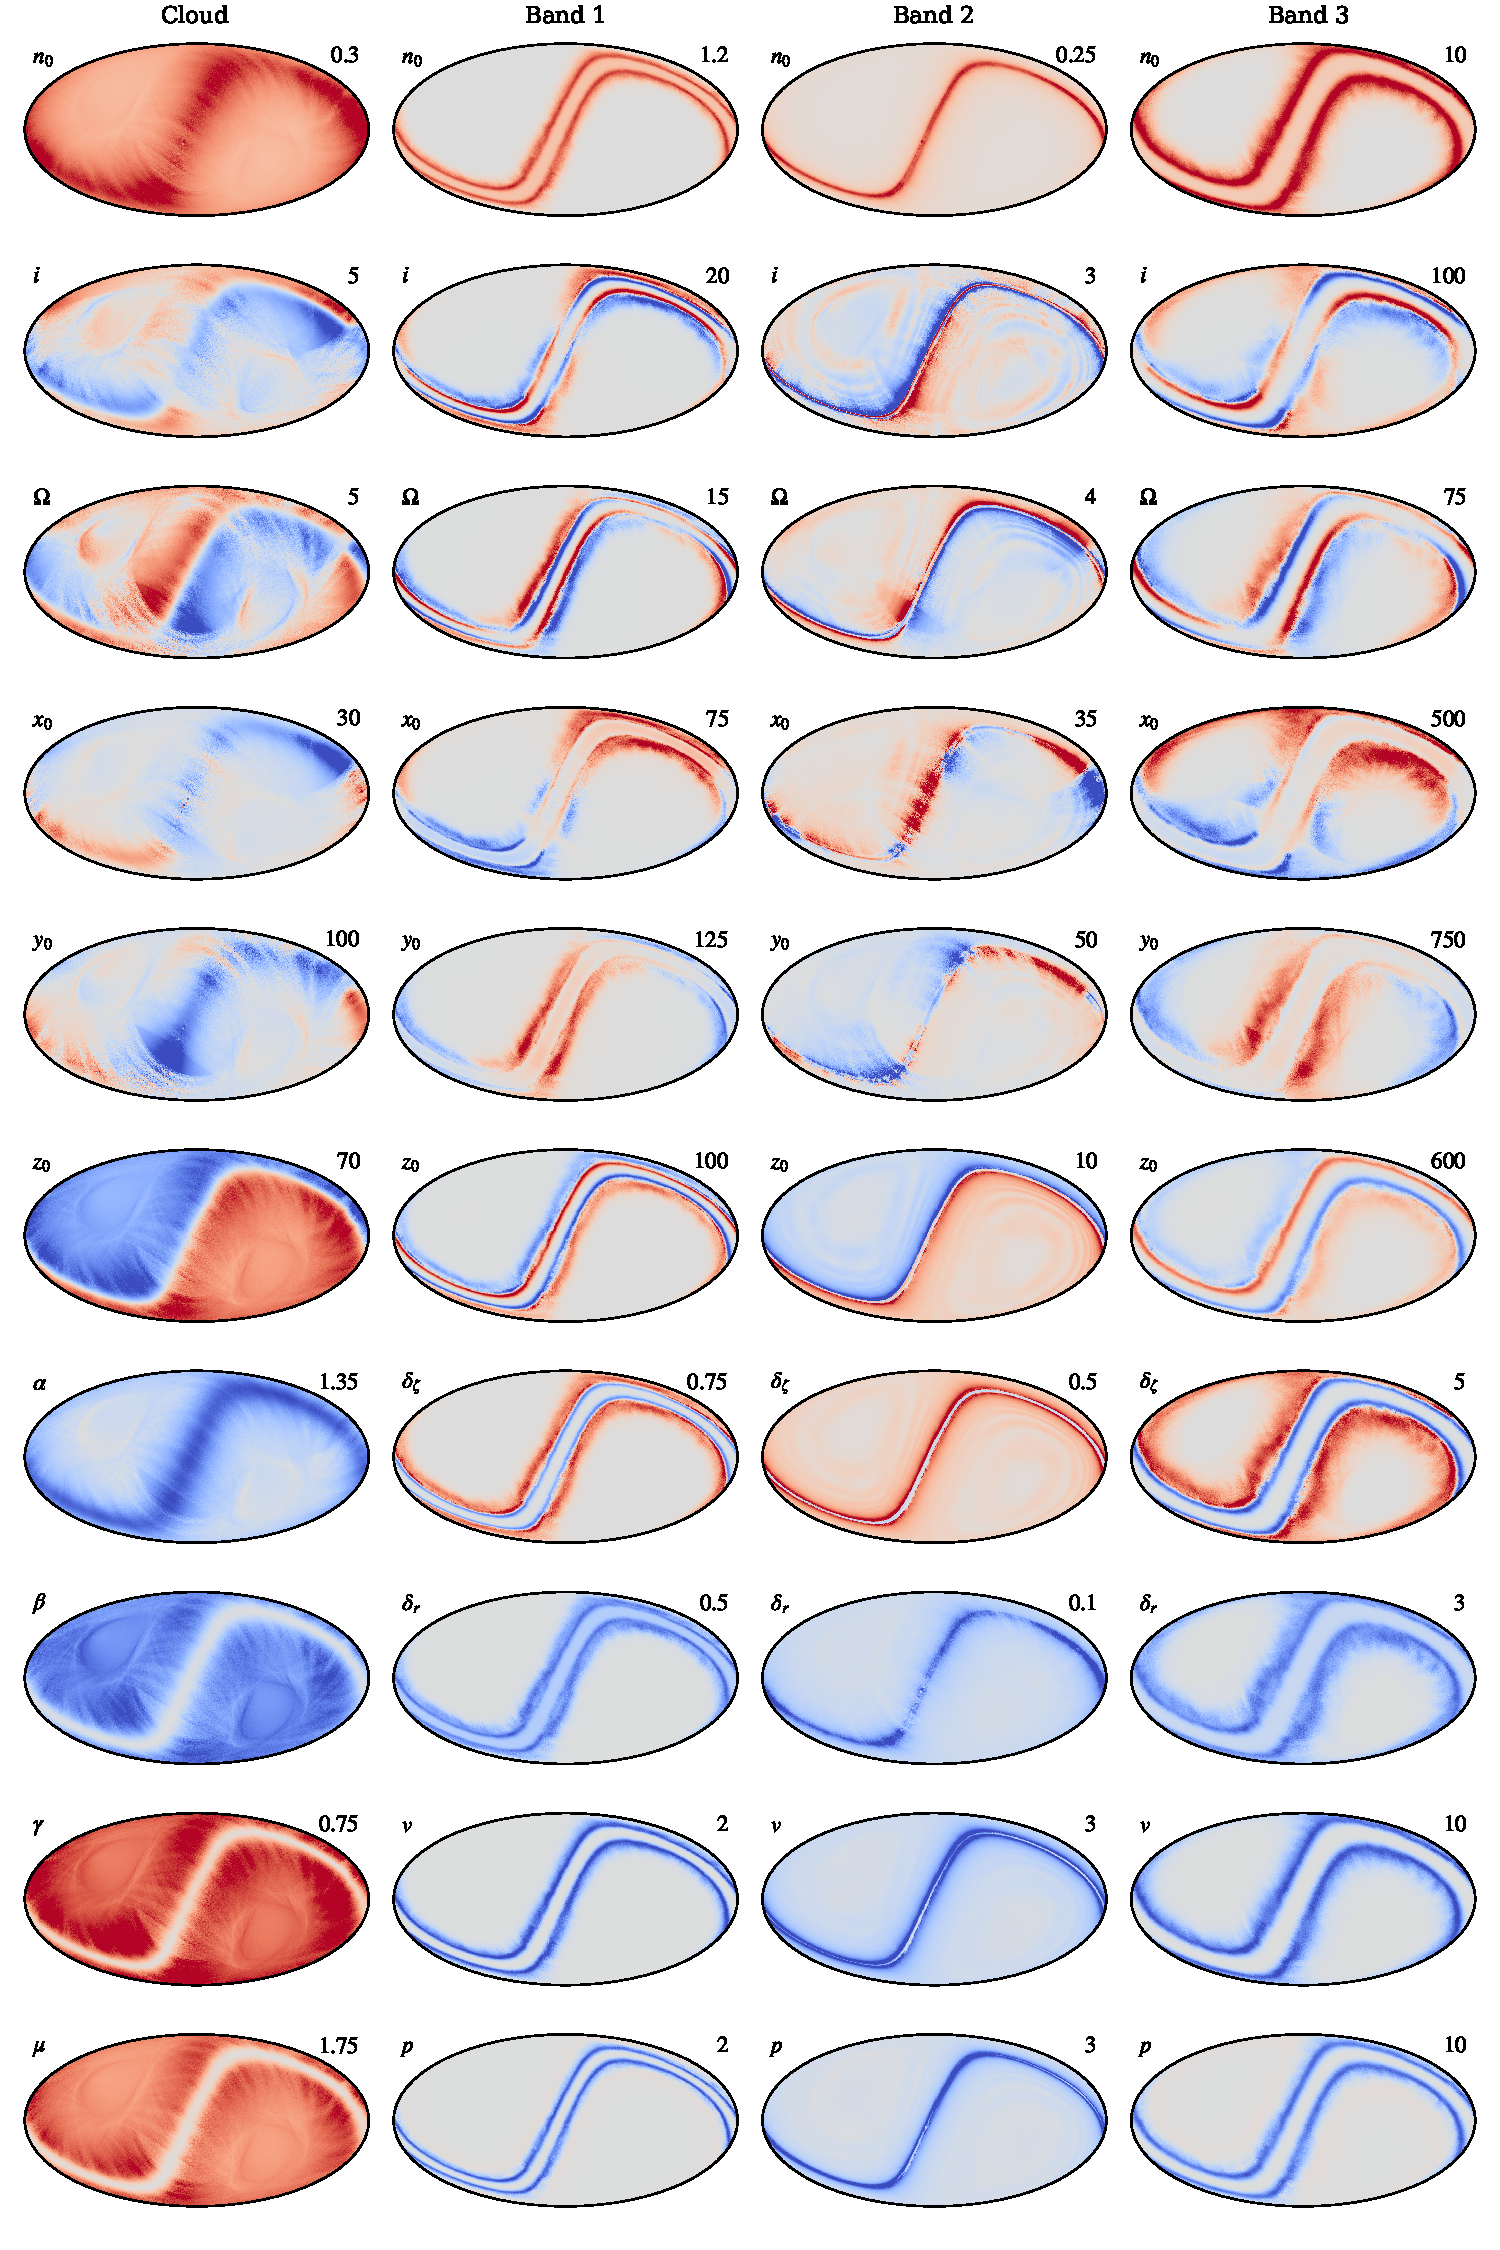
\includegraphics[width=0.8\linewidth]{figs/atlas_1_v2.pdf}
  	\caption{Atlas 1}
	\label{fig: atlas1}
\end{figure*}


\section{Conclusions}
\blindtext

\begin{acknowledgements}
 The current work has received funding from the European
  Union’s Horizon 2020 research and innovation programme under grant
  agreement numbers 819478 (ERC; \textsc{Cosmoglobe}) and 772253 (ERC;
  \textsc{bits2cosmology}). Some of the results in this paper have been derived using the HEALPix \citep{HEALPIX} package.
  We acknowledge the use of the Legacy Archive for Microwave Background Data
  Analysis (LAMBDA), part of the High Energy Astrophysics Science Archive Center
  (HEASARC). HEASARC/LAMBDA is a service of the Astrophysics Science Division at
  the NASA Goddard Space Flight Center.  
\end{acknowledgements}


%-------------------------------------------------------------
%                                       Table with references 
%-------------------------------------------------------------
%

\bibliographystyle{aa}
\bibliography{references}
\end{document}
%%%% End of aa.dem
